\subsubsection{Hardware USART driver in detail}
\label{sec:bus:design:layer1:interface:hwuart}

The hardware USART driver is designed in such a way as it takes only data via methods and returns data only via callback routines (which can be seen as events).\\

The methods provided by the driver are

\begin{enumerate}
 \item \textbf{initialize: } initializes the hw usart driver and configures it with certain parameters such as the baud rate and the callback methods triggered on event occurences.
 \item \textbf{writeByte: } takes a byte of data and transmitts it.
\end{enumerate}

and the events provided by the driver are

\begin{enumerate}
 \item \textbf{byteReceivedCallback}
 \item \textbf{byteTransmittedCallback}
 \item \textbf{byteCorruptedCallback}
\end{enumerate}

\begin{figure}[h]
\centering
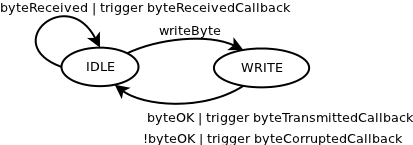
\includegraphics[width=0.8\textwidth]{../images/hwuart_statemachine.png}
\caption{Hardware USART Driver State Machine.}
\label{fig:bus:design:layer1:interface:hwuart}
\end{figure}

The workflow of the drivers statemachine depicted in figure \ref{fig:bus:design:layer1:interface:hwuart} starts in the state \textit{IDLE}.
When data is pushed into the driver via the \textit{writeByte} method the transmission via uart is initiated and the statemachine changes to state \textit{WRITE}.\\

In the state \textit{WRITE} the transmitted databyte is read back and compared with the read databyte. 
Either the read and written databytes are equal the \textit{byteTransmittedCallback} is triggered or the \textit{byteCorruptedCallback} is triggered and the statemachine leads to state \textit{IDLE}.\\

If a byte is read via the usart it is propagated via the \textit{byteReceivedCallback} event to higher layers, in the state \textit{IDLE} .\\
